%% SW design: PSoC Domain

\begin{figure}[htbp] \centering
{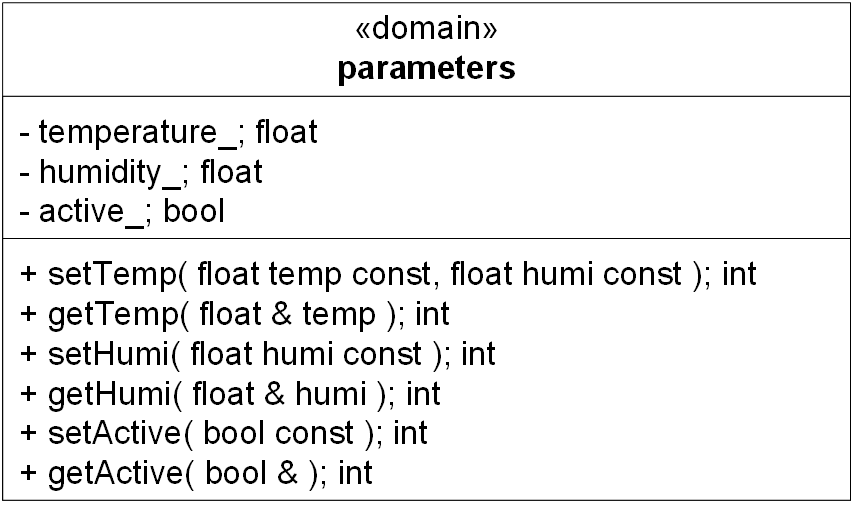
\includegraphics[scale=1.3]{filer/design/Klassediagrammer/sw_psoc_parameters}}
\caption{Klasse parameters}
\label{fig:sw_psoc_class_parameters}
\end{figure} 

{\centering
\textbf{parameters}\par
}
\textbf{Ansvar:} Gemme information om grænseværdier mv. til det autonome vandingssystem. \

\verb+int setTemp( float temp const ) +\\
\textbf{Parametre:} Temperatur. \\
\textbf{Returværdi:} 0 ved succes ellers negativ i overenstemmelse med fejl-listen. \\
\textbf{Beskrivelse:} Gemmer modtagne temperatur i medlemsdata \verb+temperature_+. \\

\verb+int getTemp( float * temp )+ \\
\textbf{Parametre:} Pointer til at gemme temperatur i. \\
\textbf{Returværdi:} 0 ved succes ellers negativ i overenstemmelse med fejl-listen. \\
\textbf{Beskrivelse:} Returnerer medlem \verb+temperature_+ i reference. \\

\verb+int setHumi( float humi const )+ \\
\textbf{Parametre:} Humidity. \\
\textbf{Returværdi:} 0 ved succes ellers negativ i overenstemmelse med fejl-listen. \\
\textbf{Beskrivelse:} Gemmer modtagne humidity i medlemsdata \verb+humidity_+. \\

\verb+int getHumi( float * humi )+ \\
\textbf{Parametre:} Pointer til at gemme humidity i. \\
\textbf{Returværdi:} 0 ved succes ellers negativ i overenstemmelse med fejl-listen. \\
\textbf{Beskrivelse:} Returnerer medlem \verb+humidity_+ i reference. \\

\verb+int setActive( unsigned char const )+ \\
\textbf{Parametre:} 1 = aktiv, 0 = inaktiv. \\
\textbf{Returværdi:} 0 ved succes ellers negativ i overenstemmelse med fejl-listen. \\
\textbf{Beskrivelse:} Gemmer modtagne char i medlemsdata \verb+active_+. \\

\verb+int getActive( unsigned char * )+ \\
\textbf{Parametre:} Pointer til at gemme unsigned char i. \\
\textbf{Returværdi:} 0 ved succes ellers negativ i overenstemmelse med fejl-listen. \\
\textbf{Beskrivelse:} Returnerer medlem \verb+active_+ i pointer. \\


\begin{figure}[htbp] \centering
{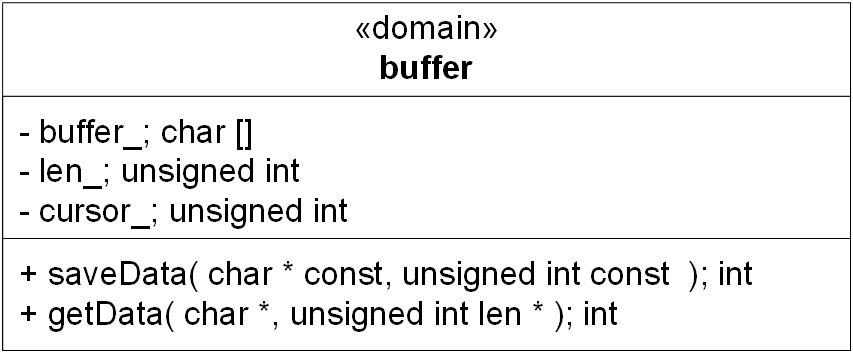
\includegraphics[scale=1.3]{filer/design/Klassediagrammer/sw_psoc_buffer}}
\caption{Klasse buffer}
\label{fig:sw_psoc_class_buffer}
\end{figure} 

{\centering
\textbf{buffer}\par
}
\textbf{Ansvar:} Holde data fra sensorerne indtil de udlæses af Master. \

\verb+buffer( )+ \\
\textbf{Parametre:} Ingen. \\
\textbf{Returværdi:} Ingen. \\
\textbf{Beskrivelse:} Skal initialisere \verb+char+ array \verb+buffer_+ med plads til én datamåling og 10 fejl iht. dataprotokol. \\

\verb+int saveData( char * buf const, unsigned int len const )+ \\
\textbf{Parametre:} Pointer til buffer med len data. \\
\textbf{Returværdi:} 0 ved succes ellers negativ i overenstemmelse med fejl-listen. \\
\textbf{Beskrivelse:} Skal gemme modtaget data i \verb+buffer_+-medlemmet og flytte \verb+cursor_+ antallet af karakterer frem.\\

\verb+int getData( char * buf, unsigned int * len )+ \\
\textbf{Parametre:} Pointer til char array til data. \\
\textbf{Returværdi:} 0 ved succes ellers negativ i overenstemmelse med fejl-listen. \\
\textbf{Beskrivelse:} Skal returnere data fra \verb+buffer_+ i pointer og nulstille \verb+cursor_+-medlemmet.\\